\providecommand{\master}{..}
\documentclass[\master/Master.tex]{subfiles}
\begin{document}

\subsection{Restrictions and simplifications}
In order to simplify the problem we have made the following restrictions on conditional effects we can learn:

\newlist{propenum}{enumerate}{1} % also creates a counter called 'propenumi'
\setlist[propenum]{label=R. \arabic*}
\crefalias{propenumi}{arestriction} 

\begin{propenum}[label=R.\arabic*]
	\item \label{rst:ca:no-action-params} Actions cannot have parameters, i.e.\ all actions are of the form $A()$. 
	We have added this restricting to study the problem in its most minimal form.	
	\item The environment must be fully observable.
	\item The environment must contain a finite number of objects.
    \item \label{rst:ca:no-disjuntive-conditionals} \label{rst:ca:no-multiple-effect} A predicate can only be part of a one negative and one positive literal in the effects of all conditionals for an action $A$. 
    
    This allows us to associate any effect literal with exactly one conditional. An additional consequence of this restriction is that disjunctive preconditions are not supported, since that would require an effect literal to occur in two different conditionals.

	\item \label{rst:ca:no-disjoint-preconditions} No disjoint preconditions.

		  A disjoint precondition is when it is not connected to an effect or another non-disjoint precondition through its variables.
		  I.e.\ If a conditional effect had the effect $p(x)$ a disjoint precondition could be $p(y)$ as $x \neq y$ however if it also had a precondition $q(x,y)$ this would connect the two variables thus making $p(y)$ non-disjoint.
\end{propenum}

When a STRIPS-style (non-conditional) action is invoked with arguments $O_1, \dots, O_n$, it is certain that these arguments are the only objects affected by the action.
Thus, any atom in a state that contains objects other than these can be discarded as irrelevant when learning either the effects or the preconditions.
However, when actions contain conditional effects with support for use of quantifiers, this claim no longer holds.
To properly discuss the subject we introduce \glits, which is the set of all grounded literals.

\begin{definition}
	All possible grounded literals \glits is defined as:
	\begin{equation*}
		\glits =
		\left\{ \neg p\left(O_1, \dots, O_{|p|}\right), 
				p\left(O_1, \dots, O_{|p|}\right) 
				\mid 
		p \in \preds \land 
		\left\{O_1, \dots, O_{|p|} \right\} \subseteq \objs
		\right\}
	\end{equation*}
	
	to avoid defining it as a function, it can be assumed that $\preds$ and $\objs$ are given from the context.
\end{definition}


Given the restrictions listed above, we are able to simplify the problem. That is, we can model every possible action schema where each conditional only contains one effect.

\begin{example} This example shows that conditionals with multiple effects can always be split into multiple conditionals, thus making modeling of the problem simpler.
	Take for instance this action with a conditional:	
	\begin{align*}
		&A():&  \\
		&\quad
		\forall_{x, y}
			\left[
				q(x) \land h(y)
			\right]
		\; when \;
		\left[ p(x,y) \right]
	\end{align*}		
	That action is equivalent to: 
	\begin{align*}
		A():&  \\
			 &\quad\forall_{x, y}
				\left[
				h(y)
				\right]
				\; when \;
				\left[ p(x,y) \right] \\
		&\quad\land 	\\		
		&\quad\forall_{x, y}
		\left[
		\texttt{q}(x)
		\right]
		\; when \;
		\left[ p(x,y) \right]
	\end{align*}
	
\end{example}

\begin{proposition}[Single effect per conditional]\label{prop:ca:singleConditional}
    Consider a state transition $\left(S, a, S'\right)$ and a grounded literal $p \in \geffects$. By \Cref{rst:ca:no-multiple-effect}, there is exactly one conditional in $A$ that could be responsible for producing $p$. Consequently, any two literals in $\geffects$ with the same predicate are effects of the same conditional.
\end{proposition}

\begin{figure}
	\centering{%
	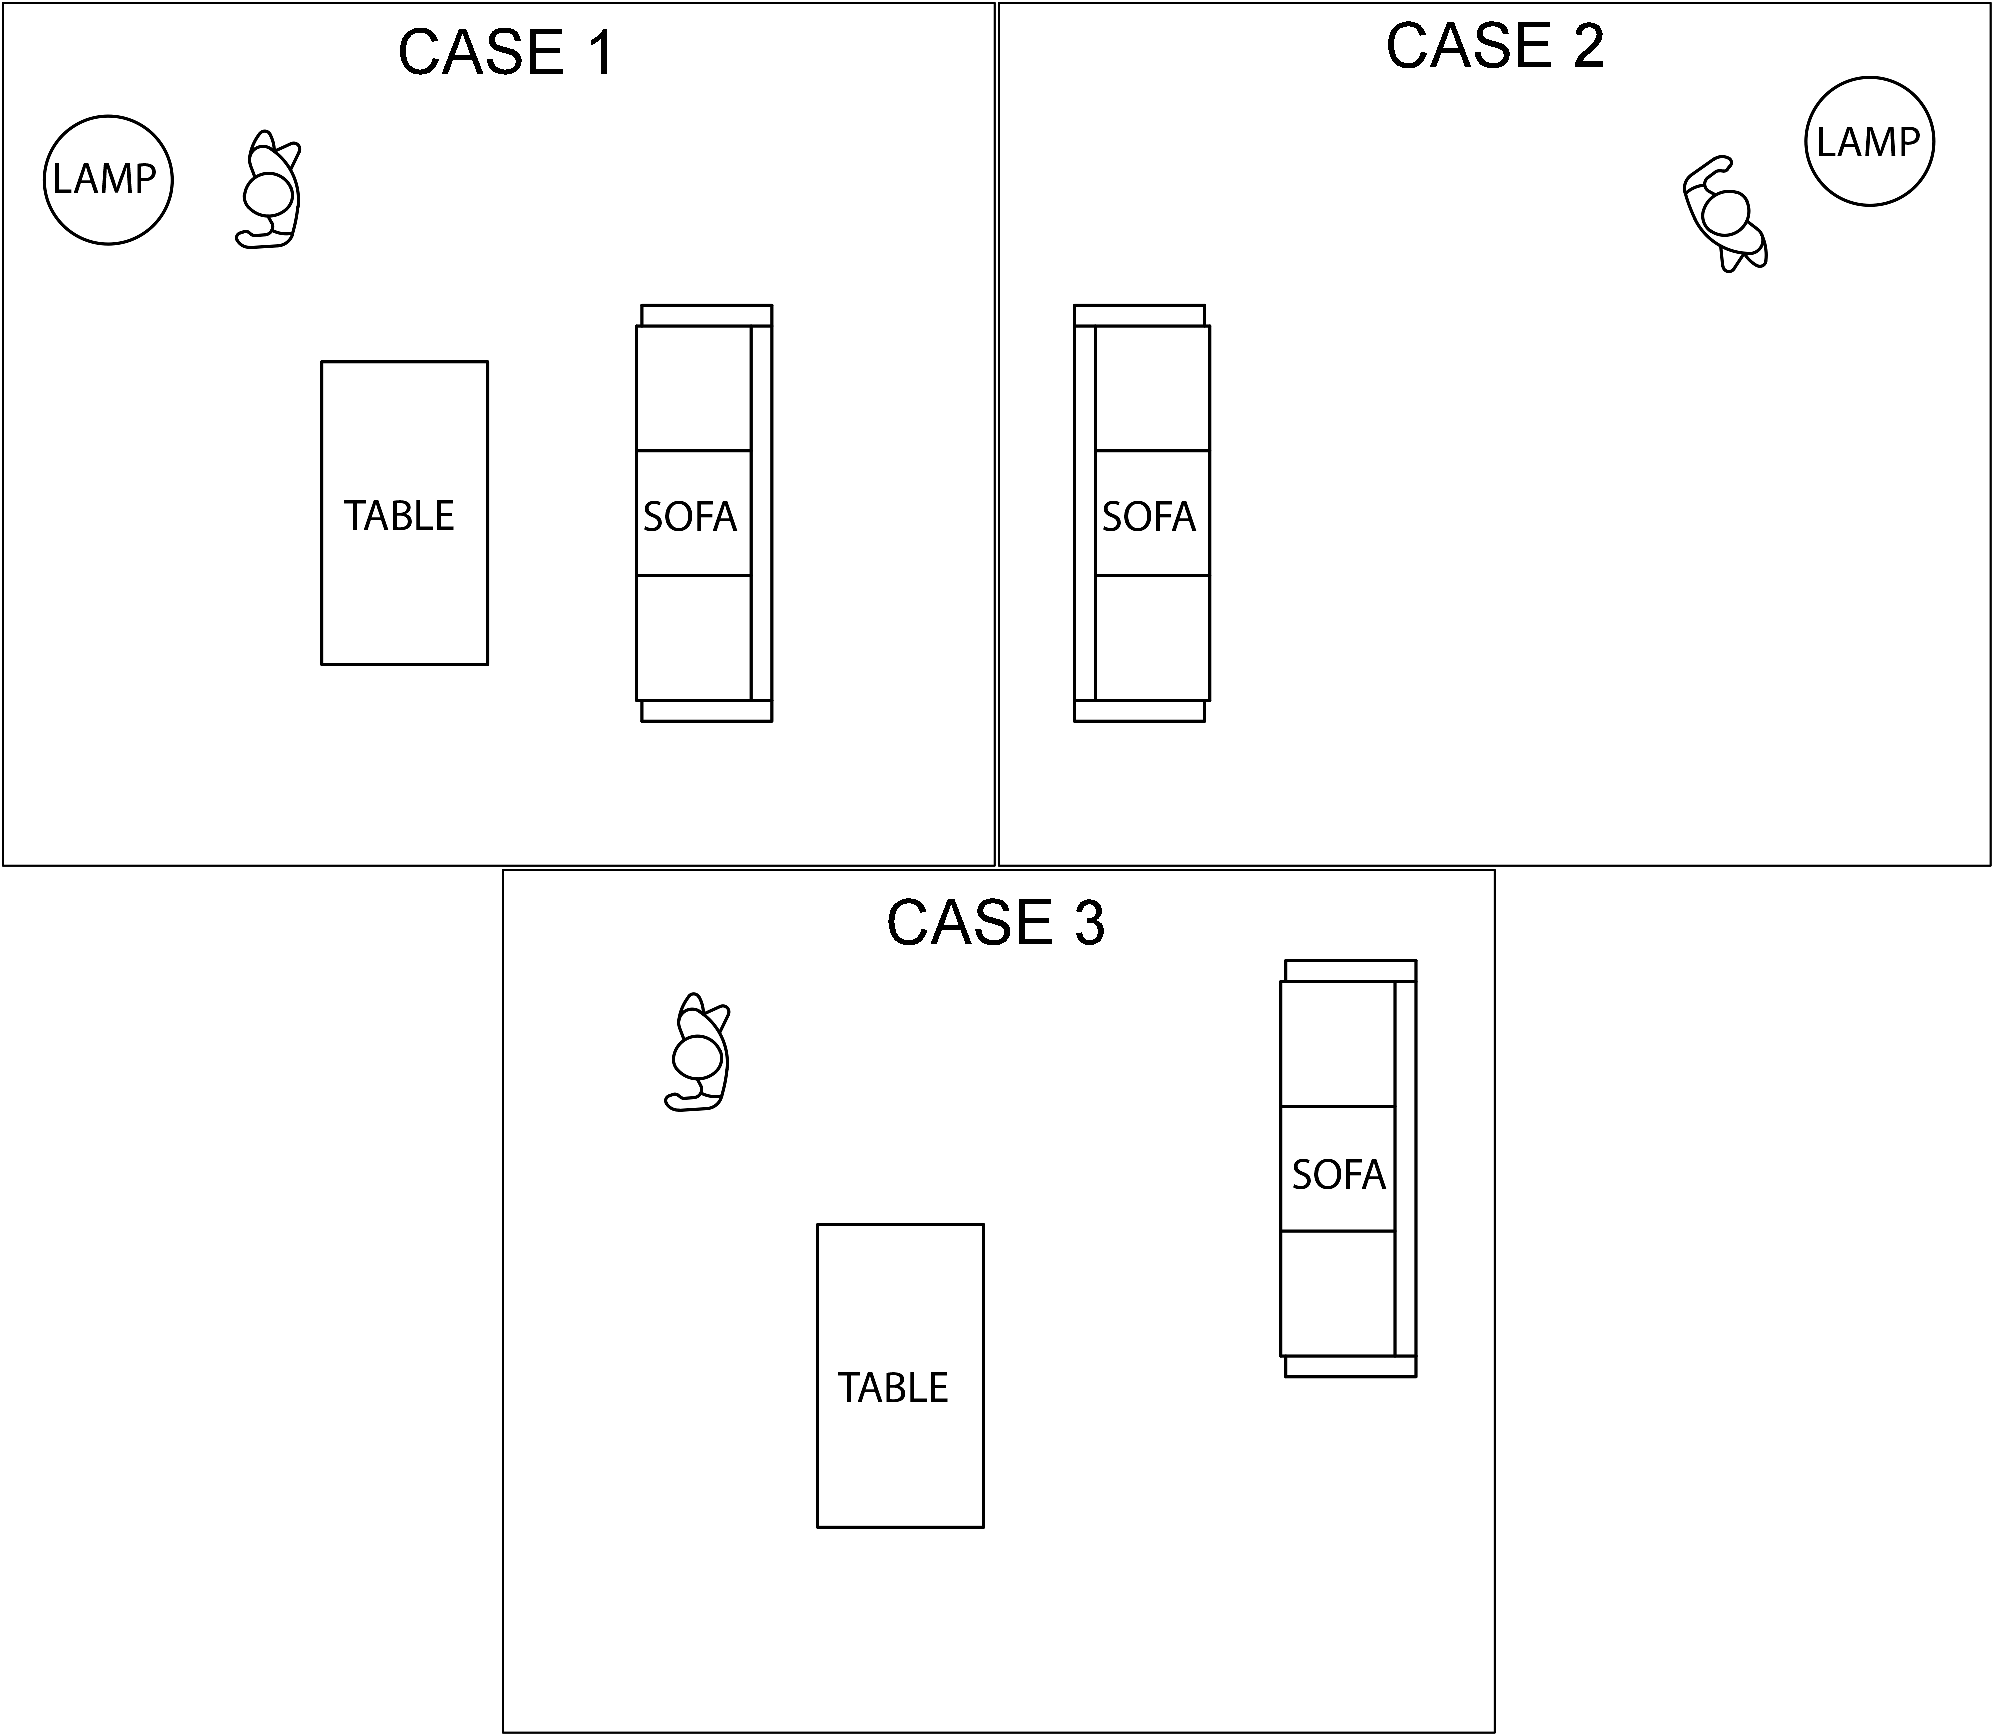
\includegraphics[width=0.7\textwidth]{\master/Graphics/house_conditional_knowledge}}
	\caption{\label{fig:ca:house-example}Three states of light problem for \Cref{ex:ca:light-on}}
\end{figure}

\subsection{Learning conditional effects}


With the above simplification of the problem, we will now analyze what it means to learn conditional effects.
It is important to realize that in a conditional effect supported domain, if we observe an effect we must assume every atom connected to that effect is part of the preconditions. Only when the we observe a contradiction to this statement can we dismiss it. 

Consider again a state transition $(S,a,S')$. Trivially, when an atom $q\left(O_1, \dots, O_{|p|}\right)$ occurs in $\Delta S$, it holds that there is a conditional in $A$ with literal $q\left(x_1, \dots, x_{|q|}\right)$ as an effect. That is, there exists a conditional of the form

\begin{equation*}
    E_C = \forall x_1, \dots, x_n 
    \left[ q\left(x_1, \dots, x_{|q|} \right) \right] \quad when \quad 
    \left[ \bigwedge_{p \in P} p \right]
\end{equation*}
where $P$ is a set of preconditions. Additionally, there exists an interpretation $\delta$ such that the observed effect is produced and the preconditions are satisfied in the state, i.e.\ $\delta\left(q\left(x_1, \dots, x_{|p|} \right)\right) \in \Delta S$ and $\delta\left[ P \right] \subseteq X(S)$. This interpretation resembles the grounding function from non-conditional learning, and similarly to non-conditional learning, the inverse can now be used with $X(S)$ to obtain a set of literals guaranteed to contain all preconditions. For conditionals, this inverse grounding function is denoted $\sigma$.

% It now holds that if we can find the inverse of such an interpretation, i.e.\ one that maps objects in $\objs$ to variables in $\varC\left(E_C\right)$, where $\delta^{-1}\left(O_1\right) = x_1, \dots, \delta^{-1}\left(O_{|q|}\right) = x_{|q|}$, then $\delta^{-1} \left[ X(S) \right]$ contains the preconditions $P$. In the following, such a mapping is called $\sigma$.

\begin{theorem}\label{thm:ca:precondition-state}
If $\gamma (S,a) = S'$ then $\pre(\sigma(e)) \subseteq \sigma(\ts(S))$\footnote{\ts(S) gives the state where atoms absent from the state are represented as negative literals, see \Cref{def:pddl:explicit-state}} for the effect $e \in \geffects$.
Therefore limiting the preconditions to literals in $\ts(S)$ is guaranteed not to remove actual preconditions.
\end{theorem}
\begin{proof}[\textbf{Proof by contradiction}] Assume that there are more preconditions than present in $\ts(S)$ for the effects \geffects.
	In this case the effects would not occur as their required preconditions are missing, thus the preconditions must be satisfied in $\ts(S)$.
	As such we can conclude $\ts(S)$ contains at least all precondition literals.
\end{proof}

\begin{figure}
	\hspace*{0.1\textwidth}%
	\begin{subfigure}{0.35\textwidth}
		\centering
		\resizebox{\linewidth}{!}{\begin{pgfpicture}
  \pgfpathrectangle{\pgfpointorigin}{\pgfqpoint{200.0000bp}{200.0000bp}}
  \pgfusepath{use as bounding box}
  \begin{pgfscope}
    \definecolor{fc}{rgb}{0.0000,0.0000,0.0000}
    \pgfsetfillcolor{fc}
    \pgftransformshift{\pgfqpoint{166.6667bp}{66.6667bp}}
    \pgftransformscale{1.6667}
    \pgftext[base,left]{$t_{3}$}
  \end{pgfscope}
  \begin{pgfscope}
    \definecolor{fc}{rgb}{0.0000,0.0000,0.0000}
    \pgfsetfillcolor{fc}
    \pgftransformshift{\pgfqpoint{100.0000bp}{66.6667bp}}
    \pgftransformscale{1.6667}
    \pgftext[base,left]{$t_{2}$}
  \end{pgfscope}
  \begin{pgfscope}
    \definecolor{fc}{rgb}{0.0000,0.0000,0.0000}
    \pgfsetfillcolor{fc}
    \pgftransformshift{\pgfqpoint{33.3333bp}{66.6667bp}}
    \pgftransformscale{1.6667}
    \pgftext[base,left]{$t_{1}$}
  \end{pgfscope}
  \begin{pgfscope}
    \definecolor{fc}{rgb}{0.0000,0.0000,0.0000}
    \pgfsetfillcolor{fc}
    \pgfsetfillopacity{0.0000}
    \pgfsetlinewidth{2.0000bp}
    \definecolor{sc}{rgb}{0.0000,0.0000,0.0000}
    \pgfsetstrokecolor{sc}
    \pgfsetmiterjoin
    \pgfsetbuttcap
    \pgfpathqmoveto{186.6667bp}{133.3333bp}
    \pgfpathqcurveto{186.6667bp}{144.3790bp}{177.7124bp}{153.3333bp}{166.6667bp}{153.3333bp}
    \pgfpathqcurveto{155.6210bp}{153.3333bp}{146.6667bp}{144.3790bp}{146.6667bp}{133.3333bp}
    \pgfpathqcurveto{146.6667bp}{122.2876bp}{155.6210bp}{113.3333bp}{166.6667bp}{113.3333bp}
    \pgfpathqcurveto{177.7124bp}{113.3333bp}{186.6667bp}{122.2876bp}{186.6667bp}{133.3333bp}
    \pgfpathclose
    \pgfusepathqfillstroke
  \end{pgfscope}
  \begin{pgfscope}
    \definecolor{fc}{rgb}{0.0000,0.0000,0.0000}
    \pgfsetfillcolor{fc}
    \pgfsetfillopacity{0.0000}
    \pgfsetlinewidth{2.0000bp}
    \definecolor{sc}{rgb}{0.0000,0.0000,0.0000}
    \pgfsetstrokecolor{sc}
    \pgfsetmiterjoin
    \pgfsetbuttcap
    \pgfpathqmoveto{200.0000bp}{100.0000bp}
    \pgfpathqlineto{200.0000bp}{166.6667bp}
    \pgfpathqlineto{133.3333bp}{166.6667bp}
    \pgfpathqlineto{133.3333bp}{100.0000bp}
    \pgfpathqlineto{200.0000bp}{100.0000bp}
    \pgfpathclose
    \pgfusepathqfillstroke
  \end{pgfscope}
  \begin{pgfscope}
    \definecolor{fc}{rgb}{0.0000,0.0000,0.0000}
    \pgfsetfillcolor{fc}
    \pgftransformshift{\pgfqpoint{100.0000bp}{133.3333bp}}
    \pgftransformscale{1.6667}
    \pgftext[base,left]{$c$}
  \end{pgfscope}
  \begin{pgfscope}
    \definecolor{fc}{rgb}{0.0000,0.0000,0.0000}
    \pgfsetfillcolor{fc}
    \pgfsetfillopacity{0.0000}
    \pgfsetlinewidth{2.0000bp}
    \definecolor{sc}{rgb}{0.0000,0.0000,0.0000}
    \pgfsetstrokecolor{sc}
    \pgfsetmiterjoin
    \pgfsetbuttcap
    \pgfpathqmoveto{120.0000bp}{113.3333bp}
    \pgfpathqlineto{120.0000bp}{153.3333bp}
    \pgfpathqlineto{80.0000bp}{153.3333bp}
    \pgfpathqlineto{80.0000bp}{113.3333bp}
    \pgfpathqlineto{120.0000bp}{113.3333bp}
    \pgfpathclose
    \pgfusepathqfillstroke
  \end{pgfscope}
  \begin{pgfscope}
    \definecolor{fc}{rgb}{0.0000,0.0000,0.0000}
    \pgfsetfillcolor{fc}
    \pgfsetfillopacity{0.0000}
    \pgfsetlinewidth{2.0000bp}
    \definecolor{sc}{rgb}{0.0000,0.0000,0.0000}
    \pgfsetstrokecolor{sc}
    \pgfsetmiterjoin
    \pgfsetbuttcap
    \pgfpathqmoveto{133.3333bp}{100.0000bp}
    \pgfpathqlineto{133.3333bp}{166.6667bp}
    \pgfpathqlineto{66.6667bp}{166.6667bp}
    \pgfpathqlineto{66.6667bp}{100.0000bp}
    \pgfpathqlineto{133.3333bp}{100.0000bp}
    \pgfpathclose
    \pgfusepathqfillstroke
  \end{pgfscope}
  \begin{pgfscope}
    \definecolor{fc}{rgb}{0.0000,0.0000,0.0000}
    \pgfsetfillcolor{fc}
    \pgfsetfillopacity{0.0000}
    \pgfsetlinewidth{2.0000bp}
    \definecolor{sc}{rgb}{0.0000,0.0000,0.0000}
    \pgfsetstrokecolor{sc}
    \pgfsetmiterjoin
    \pgfsetbuttcap
    \pgfpathqmoveto{66.6667bp}{100.0000bp}
    \pgfpathqlineto{66.6667bp}{166.6667bp}
    \pgfpathqlineto{-0.0000bp}{166.6667bp}
    \pgfpathqlineto{-0.0000bp}{100.0000bp}
    \pgfpathqlineto{66.6667bp}{100.0000bp}
    \pgfpathclose
    \pgfusepathqfillstroke
  \end{pgfscope}
\end{pgfpicture}
}
		\caption{Before execution of \texttt{MoveLeft}}
	\end{subfigure}%
	\hspace*{0.1\textwidth}%
	\begin{subfigure}{0.35\textwidth}
		\centering
		\resizebox{\linewidth}{!}{\begin{pgfpicture}
  \pgfpathrectangle{\pgfpointorigin}{\pgfqpoint{200.0000bp}{200.0000bp}}
  \pgfusepath{use as bounding box}
  \begin{pgfscope}
    \definecolor{fc}{rgb}{0.0000,0.0000,0.0000}
    \pgfsetfillcolor{fc}
    \pgftransformshift{\pgfqpoint{166.6667bp}{66.6667bp}}
    \pgftransformscale{1.6667}
    \pgftext[base,left]{$t_{3}$}
  \end{pgfscope}
  \begin{pgfscope}
    \definecolor{fc}{rgb}{0.0000,0.0000,0.0000}
    \pgfsetfillcolor{fc}
    \pgftransformshift{\pgfqpoint{100.0000bp}{66.6667bp}}
    \pgftransformscale{1.6667}
    \pgftext[base,left]{$t_{2}$}
  \end{pgfscope}
  \begin{pgfscope}
    \definecolor{fc}{rgb}{0.0000,0.0000,0.0000}
    \pgfsetfillcolor{fc}
    \pgftransformshift{\pgfqpoint{33.3333bp}{66.6667bp}}
    \pgftransformscale{1.6667}
    \pgftext[base,left]{$t_{1}$}
  \end{pgfscope}
  \begin{pgfscope}
    \definecolor{fc}{rgb}{0.0000,0.0000,0.0000}
    \pgfsetfillcolor{fc}
    \pgfsetfillopacity{0.0000}
    \pgfsetlinewidth{2.0000bp}
    \definecolor{sc}{rgb}{0.0000,0.0000,0.0000}
    \pgfsetstrokecolor{sc}
    \pgfsetmiterjoin
    \pgfsetbuttcap
    \pgfpathqmoveto{200.0000bp}{100.0000bp}
    \pgfpathqlineto{200.0000bp}{166.6667bp}
    \pgfpathqlineto{133.3333bp}{166.6667bp}
    \pgfpathqlineto{133.3333bp}{100.0000bp}
    \pgfpathqlineto{200.0000bp}{100.0000bp}
    \pgfpathclose
    \pgfusepathqfillstroke
  \end{pgfscope}
  \begin{pgfscope}
    \definecolor{fc}{rgb}{0.0000,0.0000,0.0000}
    \pgfsetfillcolor{fc}
    \pgfsetfillopacity{0.0000}
    \pgfsetlinewidth{2.0000bp}
    \definecolor{sc}{rgb}{0.0000,0.0000,0.0000}
    \pgfsetstrokecolor{sc}
    \pgfsetmiterjoin
    \pgfsetbuttcap
    \pgfpathqmoveto{120.0000bp}{133.3333bp}
    \pgfpathqcurveto{120.0000bp}{144.3790bp}{111.0457bp}{153.3333bp}{100.0000bp}{153.3333bp}
    \pgfpathqcurveto{88.9543bp}{153.3333bp}{80.0000bp}{144.3790bp}{80.0000bp}{133.3333bp}
    \pgfpathqcurveto{80.0000bp}{122.2876bp}{88.9543bp}{113.3333bp}{100.0000bp}{113.3333bp}
    \pgfpathqcurveto{111.0457bp}{113.3333bp}{120.0000bp}{122.2876bp}{120.0000bp}{133.3333bp}
    \pgfpathclose
    \pgfusepathqfillstroke
  \end{pgfscope}
  \begin{pgfscope}
    \definecolor{fc}{rgb}{0.0000,0.0000,0.0000}
    \pgfsetfillcolor{fc}
    \pgfsetfillopacity{0.0000}
    \pgfsetlinewidth{2.0000bp}
    \definecolor{sc}{rgb}{0.0000,0.0000,0.0000}
    \pgfsetstrokecolor{sc}
    \pgfsetmiterjoin
    \pgfsetbuttcap
    \pgfpathqmoveto{133.3333bp}{100.0000bp}
    \pgfpathqlineto{133.3333bp}{166.6667bp}
    \pgfpathqlineto{66.6667bp}{166.6667bp}
    \pgfpathqlineto{66.6667bp}{100.0000bp}
    \pgfpathqlineto{133.3333bp}{100.0000bp}
    \pgfpathclose
    \pgfusepathqfillstroke
  \end{pgfscope}
  \begin{pgfscope}
    \definecolor{fc}{rgb}{0.0000,0.0000,0.0000}
    \pgfsetfillcolor{fc}
    \pgftransformshift{\pgfqpoint{33.3333bp}{133.3333bp}}
    \pgftransformscale{1.6667}
    \pgftext[base,left]{$c$}
  \end{pgfscope}
  \begin{pgfscope}
    \definecolor{fc}{rgb}{0.0000,0.0000,0.0000}
    \pgfsetfillcolor{fc}
    \pgfsetfillopacity{0.0000}
    \pgfsetlinewidth{2.0000bp}
    \definecolor{sc}{rgb}{0.0000,0.0000,0.0000}
    \pgfsetstrokecolor{sc}
    \pgfsetmiterjoin
    \pgfsetbuttcap
    \pgfpathqmoveto{53.3333bp}{113.3333bp}
    \pgfpathqlineto{53.3333bp}{153.3333bp}
    \pgfpathqlineto{13.3333bp}{153.3333bp}
    \pgfpathqlineto{13.3333bp}{113.3333bp}
    \pgfpathqlineto{53.3333bp}{113.3333bp}
    \pgfpathclose
    \pgfusepathqfillstroke
  \end{pgfscope}
  \begin{pgfscope}
    \definecolor{fc}{rgb}{0.0000,0.0000,0.0000}
    \pgfsetfillcolor{fc}
    \pgfsetfillopacity{0.0000}
    \pgfsetlinewidth{2.0000bp}
    \definecolor{sc}{rgb}{0.0000,0.0000,0.0000}
    \pgfsetstrokecolor{sc}
    \pgfsetmiterjoin
    \pgfsetbuttcap
    \pgfpathqmoveto{66.6667bp}{100.0000bp}
    \pgfpathqlineto{66.6667bp}{166.6667bp}
    \pgfpathqlineto{-0.0000bp}{166.6667bp}
    \pgfpathqlineto{-0.0000bp}{100.0000bp}
    \pgfpathqlineto{66.6667bp}{100.0000bp}
    \pgfpathclose
    \pgfusepathqfillstroke
  \end{pgfscope}
\end{pgfpicture}
}
		\caption{After execution of \texttt{MoveLeft}}
	\end{subfigure}
	\hspace*{0.1\textwidth}
	\caption{\label{fig:ca:sokoban-moveleft-action}\texttt{MoveLeft} action being used in a sokoban world for \Cref{ex:ca:sokoban-moveleft-action} }
	
\end{figure}


\begin{example}\label{ex:ca:sokoban-moveleft-action}
	This example shows the idea that all preconditions are guaranteed to be in the state if an effect occurs.
 In \Cref{fig:ca:sokoban-moveleft-action} we see an example of an agent in the sokoban world pushing a box using a MoveLeft action with zero parameters.
	
	The action schema that produced the effect is:
	\begin{align*}
		&MoveLeft():&  \\
		&\quad
		\forall_{x, y}
		\left[
		\neg\texttt{sokobanAt}(y) \land \texttt{sokobanAt}(x)
		\right]
		\quad when \quad
		\left[ \texttt{adj-h}(x,y) \land \texttt{sokobanAt}(y) \right]& \\
		&\quad
		\forall_{x, y, z, b}
		\left[ \neg\texttt{at}(b,y) \land \texttt{at}(b,x) \right]
		\quad when \quad
		\left[
		\begin{gathered}
			\texttt{adj-h}(x,y) \land \texttt{adj-h}(y,z) \land \\
			\texttt{sokobanAt}(z) \land \texttt{at}(b, y)
		\end{gathered}
		\right] &
	\end{align*}
	
	The state transition that occurred:
	
	\begin{equation*}\label{eq:s_before}
		S_{before} =
		\left\{
		\begin{gathered}
			\texttt{adj-h}(t1, t2), \texttt{adj-h}(t2, t3), \\
			\texttt{at}(box,t2), \texttt{sokobanAt}(t3)
		\end{gathered}
		\right\}
	\end{equation*}
	\begin{equation*}
		S_{after} =
		\left\{
		\begin{gathered}
			\texttt{adj-h}(t1, t2), \texttt{adj-h}(t2, t3), \\
			\texttt{at}(box,t1), \texttt{sokobanAt}(t2)
		\end{gathered}
		\right\}
	\end{equation*}
	The effects of the state transition we calculate:
	\begin{equation*}
		\Delta S =
		\left\{
		\begin{gathered}
			\texttt{at}(box, t1), \texttt{sokobanAt}(t2), \\
			\neg\texttt{at}(box,t2), \neg\texttt{sokobanAt}(t3)
		\end{gathered}
		\right\}
	\end{equation*}
	To interpret the objects as variables we provide some mapping of objects to variables, such a mapping could be:
	\begin{equation*}
		\delta =
		\left [
		\begin{gathered}
			t1 \mapsto x \\
			t2 \mapsto y \\
			t3 \mapsto z \\
			box \mapsto b
		\end{gathered}
		\right ]
	\end{equation*}
	We apply the mapping to the objects of $S_{before}$:
	\begin{equation*}
		\sigma(S_{before}, \delta) =
		\begin{gathered}
			\left\{
			\begin{gathered}
				\texttt{adj-h}(\delta (t1), \delta (t2)), \\
				\texttt{adj-h}(\delta (t2), \delta (t3)), \\
				\texttt{at}(\delta (box),\delta (t2)), \\
				\texttt{sokobanAt}(\delta (t3))
			\end{gathered}
			\right\}
			=
			\left\{
			\begin{gathered}
				\texttt{adj-h}(x, y), \\
				\texttt{adj-h}(y, z), \\
				\texttt{at}(y), \\
				\texttt{sokobanAt}(z)
			\end{gathered}
			\right\}
		\end{gathered}
	\end{equation*}
	We also apply the mapping to the effects $\Delta S$
	\begin{equation*}
		\sigma(\geffects, \delta) =
		\left\{
		\begin{gathered}
			\texttt{at}(\delta (box),\delta (t1)), \\
			\texttt{sokobanAt}(\delta (t2)), \\
			\neg\texttt{at}(\delta (box),\delta (t2)), \\
			\neg\texttt{sokobanAt}(\delta (t3))
		\end{gathered}
		\right\}
		=
		\left\{
		\begin{gathered}
			\texttt{at}(b,x),
			\texttt{sokobanAt}(y), \\
			\neg\texttt{at}(b,y),
			\neg\texttt{sokobanAt}(z)
		\end{gathered}
		\right\}
	\end{equation*}
	
	The resulting literals of $S_{before}$ and $\geffects$ are the preconditions and the effects.
	Therefore our hypothesis of the action scheme is:
	\begin{align*}
		&MoveLeft_{hyp}():&  \\
		&\quad
		\forall_{x, y, z, b}
		\left[
		\begin{gathered}
			\texttt{at}(b, x) \land \texttt{sokobanAt}(y) \land \\ \neg\texttt{at}(b,y) \land \neg\texttt{sokobanAt}(z) \quad
		\end{gathered}
		\right]
		when
		\left[
		\begin{gathered}
			\quad \texttt{adj-h}(x, y) \land \texttt{adj-h}(y, z) \land \\ \texttt{at}(b,y) \land \texttt{sokobanAt}(z)
		\end{gathered}
		\right]&
	\end{align*}
	
	According to \Cref{thm:ca:precondition-state} we can use $MoveLeft_{hyp}$ on $S_{before}$ and get $S_{after}$.
	\begin{align*}
		&\gamma(S_{before},MoveLeft_{hyp}) =
		\left\{
		\begin{gathered}
			\texttt{adj-h}(t1, t2), \texttt{adj-h}(t2, t3), \\
			\texttt{at}(box,t1), \texttt{sokobanAt}(t2)
		\end{gathered}
		\right\}
		= S_{after}
		&
	\end{align*}
	
	We observe that this is indeed correct.
\end{example}

While the above holds for a single effect of a conditional $E_C$ of an action schema $A$, there can be several effects produced by that conditional in a single state transition. For all of these effects we can disprove knowledge (as described above), thereby obtaining an expression for the unproven preconditions. However, combining the knowledge for several different effects is not straightforward, as each of their effects and preconditions involve different objects. The significant part of the knowledge they describe, and the part they must be compared by, is \emph{how} the relations making up their preconditions are interconnected. As such, the preconditions should be compared on the patterns their relations describe rather than the names of their variables, as those are arbitrarily chosen. To gain an intuitive understanding of this, see Example~\ref{ex:ca:light-on}.

\begin{example}\label{ex:ca:light-on} To get an idea of what it means to learn conditional effects,
consider the problem of turning on light as shown in \Cref{fig:ca:house-example}.
In the figure there are three different cases of a person learning how to turn on the
light. In the first two cases the agent successfully turns on the light while in the last nothing occurs.

In the first case we learn that to turn on the light there are these possible precondition:
\begin{itemize}
	\item There must be a sofa in the north-east corner.
	\item There must be a lamp in the north-west corner with an agent on the same spot.
	\item There must be a table in the middle.
\end{itemize}
Even though we intuitively know that it is only the lamp which is the only required object in this room for the light to turn on, we cannot discard any of the other objects present as not being a precondition.


	In the second case in \Cref{fig:ca:house-example},
	we see that we can turn on the light again but this time the sofa and the lamp has changed location and
	there is no table. From this we expand our knowledge by learning:
	\begin{itemize}
		\item Sofa and lamp location does not matter
		\item A table is not needed
	\end{itemize}
    
    Observe that although this is an abstract example, the various preconditions at each step can be seen as patterns: The exact position of the agent and the lamp do not matter, as long as they are equal. The fact that the sofa changed place means that its relation to the other objects changed from the first case, and as such it can be excluded from the pattern and the precondition.

	Its important to note that since we have not seen an absence of a sofa we cannot rule out that the presence of a sofa is a precondition for the light to turn on. This is important because it shows us that by trying different scenarios we reduce the incorrect preconditions. 

\end{example}

\subsection{Disproving preconditions}
In \Cref{ex:ca:light-on}  we saw that different objects in a room could be possible preconditions for the effect of turning on a light. But since 
objects are defined by the atoms in the state which they satisfy. As such when we say that the objects are assumed to be possible preconditions for specific effects to occur, what we are actually saying is that a specific composition of literals is the requirement for the effects to occur.
This means if we interpret the objects as variables connecting the literals in a pattern, then we can get an initial set of preconditions by using the state $S$ which led to the effects. In real terms interpreting objects as variables means mapping each object 
to a to different variable.
\begin{equation}\label{eq:ca:substitution}
	\sigma(P,\delta) =  \left\{p\left(\delta(O_1),\ldots,\delta(O_n) \right) \mid p(O_1,\ldots,O_n) \in P  \right\}
\end{equation}
For instance for the state.
$\{ p(O_1), p(O_2),\ldots,p(O_n)\}$ using a mapping
\begin{equation*}
\delta = \{O_1 \mapsto v_1, O_2 \mapsto v_2 \ldots, O_n \mapsto v_n\}
\end{equation*}
where $(v_1, v_2,\dots,v_{n-1},v_n)$ are variables for the quantifier of the conditional effect; Interpreting this state's objects as variables means to apply this mapping to the state's objects
\begin{equation*}
\{ p(\delta(O_1)), p(\delta(O_2)),\ldots,p(\delta(O_n))\} = \{ p(v_1), p(v_2),\ldots,p(v_n)\}
\end{equation*}
To see how it works in sokoban see \Cref{ex:ca:sokoban-moveleft-action}

Another property we can take advantage of is that similar to non-conditional preconditions, if an effect is successfully added to the state then that disproves all preconditions not currently satisfied.
This gives us the following:



\subsection{Initial approach to reducing preconditions}\label{ssec:ca:init-approach}

All the preconditions we get from a state can be seen as the unproven preconditions, like they were for non-conditional knowledge.
Therefore as different scenarios are explored the unproven set $\Up_p$ of preconditions can be reduced.

\begin{definition}
The unproven set $\Up_p$ is the preconditions which has neither been proven nor disproven, initially it contains all  literals $\glits$.
\end{definition}

We will now consider how this unproven set can be constructed using the methods for proving and disproving preconditions presented in \Cref{sec:NC:Preconditions}, show why it is insufficient and introduce a new model which fits the domain better.

By \Cref{rst:ca:no-disjuntive-conditionals} and \Cref{rst:ca:no-multiple-effect}, each literal $p \in \geffects$ is spawned by exactly one conditional. As such, it can be deduced that if a literal $p\left(u_1, \dots, u_{|p|}\right)$ (where $\left\{u_1, \dots, u_{|p|}\right\} \subseteq \objs$) occurs in $\geffects$ after application of $a$, then $A$ contains a conditional of the form

\begin{equation*}
    \forall x_1, \dots, x_n 
        \left[ p\left(\delta\left(u_1\right), \dots, \delta \left(u_{|p|}\right) \right) \right] \quad when \quad 
        \left[ \left<unknown\right> \right]
\end{equation*}
where $\left\{\delta \left( u_1 \right), \dots, \delta \left(u_{|p|} \right) \right\} \subseteq \left\{ x_1, \dots, x_n \right\} \subseteq \delta [\objs]$ and $\delta$ is a substitution function as explained in \Cref{eq:ca:substitution}. Observe that once this conditional has been proven to exist, the problem of finding its preconditions is similar to finding the preconditions of a non-conditional action schema $A'$ accepting as many parameters as the number of objects in the world, ie. 

\begin{align*}
    \begin{split}
        \textsc{Action} &\; \textit{A'}\left(\delta \left( o_1 \right), \ldots, \delta \left( o_{|\mathcal{O}|}\right)\right): \\
        \textsc{Pre}: \; & \left< unknown \right> \\
        \textsc{Eff}: \; & p\left( \delta \left(u_1\right), \dots, \delta \left( u_{|p|} \right)\right)
    \end{split}
\end{align*}

in which case the grounding function becomes $\delta^{-1}$. Thus, the function $\dsp(S)$ from \Cref{sec:NC:Preconditions} can be used to disprove preconditions, and the set of unproven literals to be preconditions becomes $\sigma(\glits) \setminus \dsp(s)$.

As all literals in $\geffects$ with the same name are effects of the same conditional, it is tempting to consider them different applications of $A'$ and prove knowledge about their preconditions as in \Cref{sec:NC:Preconditions}. However, the above only holds for a single grounded literal observed to be the effect of the conditional; if a literal with the same predicate but different arguments occurs in $\geffects$, then it is the effect of another interpretation of the universal quantifier in the conditional, and the nonconditional action schema constructed for it will not equal $A'$.

Consequently, the preconditions disproven by $\dsp(S)$ for $A'$ are only applicable to the grounded literal $A'$ was constructed for. To find the preconditions of the conditional, a method of combining the different disproven literals is needed.

It follows from the above that if we have the sets of unproven preconditions $\Up_p1$ and $\Up_p1$ from two different state transitions, we can compare them and remove discrepancies by intersection:

\begin{equation}
\label{eq:unknownpredcondset}
	\Up_p' = \Up_p1 \cap \Up_p2
\end{equation}

\eqref{eq:unknownpredcondset} will work for removing  disproven literals only if the two sets' variables match up perfectly. Herein lies the problem of reducing preconditions; unlike non-conditional effects where variables always match with the object such that entire literals could be removed at a time, for conditional effects a reduction in the preconditions can simply mean the removal of a binding between two variables. For instance, $p(x)$ and $q(x)$ have a binding since both have the variable $x$, to remove the binding simply rename one of their variables. I.e $p(x)$ and $q(y)$.

\begin{definition}[Binding]\label{def:ca:binding}
    A binding between variables, means that variables between atoms are the same.
	Bindings that contain only one variable are disjoint and means that no binding exists.
	It is important to note that a literal with multiple variables can have bindings with itself.
	For instance $q(x)$ and $p(x,y)$ has a binding on their first argument as they both refer to the same variable, and $y$ is a disjoint variable as no other literals with $y$ exists.
\end{definition}
Therefore the approach to modeling the unknown preconditions, which we used for non-conditional actions is incorrect when used for conditional actions. See \Cref{ex:ca:nonbinding-intersection-model} for more details.



\begin{example}\label{ex:ca:nonbinding-intersection-model}
    To elucidate the problem of bindings further, imagine that we have two different $\Up_p$
    \begin{align*}
        \Up_p1 &= \{ \texttt{p}(x, x, x) \} \\
        \Up_p2 &= \{ \texttt{p}(x, x, y) \}
    \end{align*}
    We see that $\Up_p1$ has a stronger precondition, meaning that if $\Up_p1$ holds then so does $\Up_p2$ but not oppositely. I.e.\ 
    \begin{equation*}
    \texttt{p}(x, x, x) \vDash \texttt{p}(x, x, y)  \quad and \quad
     \texttt{p}(x, x, y) \nvDash \texttt{p}(x, x, x) 
    \end{equation*}
    And if we were to take the intersection between the two sets then the resulting set would be the empty set which is incorrect.
    \begin{equation*}
    	\Up_p1 \cap \Up_p2 = \emptyset
    \end{equation*}
    
     As they have the similarity of having the same binding between the first and second argument. 
     What we actually need is to have a special atom intersection $(\cap)$ that take two sets of bindings and take the intersection of that.
     \begin{equation*}
     	\Up_p1 (\cap) \Up_p2 = \{ \texttt{p}(x, x, y) \}
     \end{equation*}
\end{example}

\subsection{A new model: Connecting paths}\label{ssec:ca:connecting-paths}
From the discussion in \Cref{ssec:ca:init-approach}, 
it is evident that the model used for preconditions of non-conditional actions is not sufficient for our needs. 
Specifically, it does not allow us to easily combine knowledge obtained about the same conditional from different interpretations. 
The problem, as shown in \Cref{ex:ca:nonbinding-intersection-model}, is that this approach compares sets of literals to prove and disprove preconditions, and determines equality of the literals based on variable naming. 
However, the variable names are arbitrary and only interesting in that they describe how literals in a set are connected to each other, since it is this connectivity that determines preconditions.

In the following, we will explain a model based solely on connectivity between literals. To begin with, we will explore how literals can be connected:

\begin{definition}[Binding connection]\label{def:ca:bindingConn}
    A binding connection between indices $i$ and $j$ of two literals $p$ and $q$ means that the variable or object at the $i$'th argument of $p$ is the same as that at the $j$'th argument of $q$. In the following, the shorthand $p_i \bc q_j$ is used to denote binding connections.
    For instance, $p(x,y)$ and $q(z,x)$ has a binding connection on $p_1$ and $q_2$ since they both have $x$ on those argument indices.
    
\end{definition}

\begin{definition}[Atom connection]\label{def:ca:predicateConn}
    Similarly, the notation $p_1 \pc p_2$ denotes the rather obvious fact that the first and second argument of $p$ are both part of the same atom $p$. I.e $p(x,y)$ has an atom connection as $p_1$ and $p_2$ belong to the same atom.
\end{definition}

\begin{definition}[Combined connection]\label{def:ca:combinedConn}
	We define $p_1 \rsc p_2$ in the case that a connection is both $\pc$ and $\bc$.
	For instance $p(x,x)$ have a combined connection $p_1 \rsc p_2$. Note that it still contains all the permutations of the other connection types.
\end{definition}

Although \Cref{def:ca:predicateConn} seems insignificant, it allows us to define transitive connectivity: If $p_i \pc p_j$ and $p_j \bc q_k$ then $p_i$ and $q_k$ are connected through $p_j$. This connectivity is called a \emph{connecting path} and is denoted $p_i \pc p_j \bc q_k$.

\begin{definition}[Connecting path]\label{def:ca:connectingPath}
    A connecting path is a sequence of binding and atom connections, where any two adjacent connections shares a component, i.e.\
    \begin{equation*}
        \left< 
            \left( f_i \bc p_j \right), 
            \left( p_j \pc p_k \right), 
            \left( p_k \bc q_l \right) 
        \right>
    \end{equation*}
    where the following is used as a shorthand:
    \begin{equation*}
        f_i \bc p_j \pc p_k \bc q_l
    \end{equation*}
\end{definition}



Given a state transition $\left(S, a, S'\right)$, it now holds that for any effect $p \in \geffects$ there exists one or more connecting paths between any argument of $p$ and any argument of any literal $q \in \ts(S)$. Any one of these paths describe a possible precondition, and the set of all paths comprises the set of unproven preconditions $\Up$ for $p$. 

If another effect with the same name as $p$ occurs in $\geffects$, we can now intersect their two path sets to arrive at a correctly merged precondition set $\Up'$.

\begin{example}\label{ex:ca:non-binding-interesction-model-fixed}
	In this example we will see how connecting paths are derived from a transition and how they solve the intersection problem shown in \Cref{ex:ca:nonbinding-intersection-model}, to simplify the example we exclude negative literals.
   Let assume we have a transition (S,a,S')
   \begin{align*}
	   	S &= \{ p(A,A), g(B) \}\\
	   	S'& = S \cup \{ q(A,B) \}
   \end{align*}
   with the effect 
	\begin{equation*}
	 	\geffects = \{ q(A) \}
	\end{equation*}
	This means that from $q(A)$ we have the following connecting paths
	\begin{align*}
		\Up_0= 
		\left\{
		\begin{gathered}
			q_1 \bc p_1
		,\\	q_1 \bc p_2
		,\\	q_1 \bc p_1 \bc p_2
		,\\	q_1 \bc p_2 \bc p_1
		,\\	q_1 \pc p_1 \pc p_2 
		,\\	q_1 \pc p_2 \pc p_1 
		,\\	q_1 \bc p_1 \rsc p_2 
		,\\	q_1 \bc p_1 \rsc p_2 
		,\\ q_1 \bc g_1	
		\end{gathered}	
		\right\}	
	\end{align*}
   these connecting paths would that define our initial unproven set $\Up_0$.
   Assume that we have another unproven set $Up_1$ which is based on the $p(x,y)$ precondition which similar to the one shown in~\Cref{ex:ca:nonbinding-intersection-model}, but scaled down as .
   \begin{align*}
   	\Up_1=
   	\left\{
   	\begin{gathered}
   		 q_1 \bc p_1 
   	\end{gathered}	
   	\right\}	
   \end{align*}
   
   Intersection of $\Up_0$ and $\Up_1$ will be
	   \begin{align*}
	   	\Up_0 \cap \Up_1=
	   	\left\{
	   	\begin{gathered}
	   		q_1 \bc p_1 
	   	\end{gathered}	
	   	\right\}	
	   \end{align*}
   which is the same as $p(x,y)$. We see that the intersection now correctly reduces the literals to a single literals.
   That was unachievable in \Cref{ex:ca:nonbinding-intersection-model}.
   
   
   
   
\end{example}

\subsection{Proving preconditions}
Another aspect of learning is to determine what the actual preconditions are.
For non-conditional actions proving the preconditions of an action was a matter of using failed actions to make a list of candidate literals that through elimination eventually got down to just one literal which is then proclaimed proven. The approach is similar for conditional actions however instead of having candidates of literals; conditional actions must maintain a candidate set for the connecting paths instead of entire literals, and thus is only capable of proving a single path at a time.

\begin{theorem}\label{thm:minimum-one-binding}
    If a conditional has been observed to produce an effect (in the form of a grounded literal $p$), and failed to produce another grounded literal, then there must exist at least one connecting path from $p$ which is a precondition for that conditional.
\end{theorem}

\begin{proof}[\textbf{Proof by contradiction}] 
    If there is less than one path in the preconditions then that means there are zero paths. By \Cref{rst:ca:no-disjoint-preconditions}, zero paths means zero precondition. If there are zero preconditions then the effect would not have failed. Therefore there must be a minimum of one path that is a precondition.
\end{proof}

To discuss this we will redefine $\Up$ to be our set of possible paths, which is our set of unproven preconditions for the effect of a conditional.
If we then see that an effect does not occur in the state, the paths in the prior state that was not satisfied becomes the candidates of possible bindings $\Cand$. 

To understand this idea, see this as an almost identical solution to preconditions for non-conditional effects, but instead of literals we have paths.

Because of \Cref{thm:minimum-one-binding} the following invariant holds:
\begin{equation} \label{eq:binding_invariant}
\left| \{path  \mid  path \in \Cand \land path \in preconds_{paths}(A)\} \right|  \ge 1
\end{equation}


Meaning that at least one of the paths in this set is part of the paths in the preconditions for the conditional. As paths that are not contained in $\Up$ are disproven, we can filter disproven candidates by:
\begin{equation}
    \Cand' = \Cand \cap \Up
\end{equation}
And thus if ever $|\Cand| = 1$ then we know that it is a correct binding because of our \Cref{eq:binding_invariant} and thus it is proven.

\begin{example}\label{ex:ca:light-on-3}
    Consider the last case in \Cref{fig:ca:house-example}. This case is identical to the first case except it does not have a lamp, thus we learn that:
    \begin{itemize}
        \item A lamp is required for the effect to occur.
    \end{itemize}
    Up until this transition we have not seen proof that the lamp was a precondition even though it would be intuitive for a human that still does not mean that we can simply assume it could be that the person's action simply creates a lamp which it then proceeds to turn on, and it was the case that no lamp was created since it was present already.
    
    Interestingly like with non-conditional preconditions we require failed actions to determine the actual preconditions but unlike non-conditional preconditions an action can both succeed and fail in the same step. For instance the light was successfully turned on for the lamp but it was unsuccessful in turning on the light for the sofa.

\end{example}

\end{document}
